%!TEX root = ../TTK4900-MHT.tex
\chapter{Results}\label{chapter:results}
The performance evaluation of any tracking system difficult since the degrees of freedom are very large and there are no single of few obvious performance metrics. There are however two distinct found in the literature, pure Monte Carlo testing and situation / scenario testing. The first being that parameters like number of tracks, start position, velocity, manoeuvring, missed detections and clutter all are randomly selected and repeated many times. From a pure numerical point of view this approach seems reasonable, but it does not necessary create realistic tracking scenarios for observation dimensions higher that one. The second approach to testing is to create one or more scenarios which then is simulated with random variables like detection and noise. This approach is vulnerable to the created scenarios, since the design can heavily impact the measured performance. This method allows also for construction of very specific situations where it is desirable to test multiple tracking system on the same custom created situation for comparison purposes.

\section{Testing scheme}
The performance evaluation of any MHT system is tedious in that it is necessary to test very many different situations to get a good understanding of how the system is performing. The two largest factors contributing to the difficulty is the random nature of the clutter and lost detections. It is also desirable to evaluate the initialization and tracking performance under both varying environmental (external) conditions and tuning (internal) setting. We want good tracking of targets with low probability of detection in cluttered environment, and secondly it must be able to do this within the time frame of the radar rotation period. The initialization module must be able to detect targets with probability of detection lower than unity without initializing too many false tracks into the MHT algorithm. The testing is separated into two parts; initialization and tracking.

The performance metrics for the initialization module is how long time it takes to initialize the correct tracks, which is tested under a range of internal and external conditions, see (\ref{eq:init_test_table}). All combinations of these parameters were simulated on all scenarios (Table~\ref{tab:ais_scenarios}), which are the same routes but with different \gls{ais} configurations. 
 From these simulations, the time to initiate true targets and amount of erroneous targets are calculated. A track is categorized as correct initialized if the state difference between the true track and the initial track is less that a threshold. All initial tracks that does not correspond to a true track is categorized as erroneous. To analyse the impact of the erroneous tracks, the lifespan of falsely initiated tracks is plotted to see whether they die out at the same rate as they are initiated, or if they accumulate.
\begin{equation}\label{eq:init_test_table}
\begin{split}
\V{P_D} &= \begin{bmatrix} .9 & 0.8 & 0.6 \end{bmatrix} \\
(m/n) &= \begin{bmatrix} 	(1/1) & (1/2) & (1/3) & (1/4) \\
							(2/2) & (2/3) & (2/4) & (2/5) \\
							(3/3) & (3/4) & (3/5) & (3/6)
		   \end{bmatrix} \\
\V{\lambda_\phi} &= \begin{bmatrix} 0 & 5\cdot10^{-6} & 1\cdot10^{-5}\end{bmatrix}
\end{split}
\end{equation}

When testing the tracking performance, it is desirable to remove the variable of initialization to better see difference in \emph{tacking} rather than \emph{initialization}. All simulations testing tracking performance are carried out with all targets correctly initialized at initial time, and with the initiator set to \( (2/4) \) such that the unused measurements from the tracking algorithm would be treated as normal. This would also give lost targets a change to get re-initialized, which is an important property for any safety critical system.
\begin{equation}\label{eq:tracking_test_table}
\begin{split}
\V{P_D} &= \begin{bmatrix} .9 & 0.8 & 0.6 \end{bmatrix} \\
\V{N} &= \begin{bmatrix} 1 & 3 & 6 & 9 \end{bmatrix} \\
\V{\lambda_\phi} &= \begin{bmatrix} 0 & 5\cdot10^{-6} & 1\cdot10^{-5} \end{bmatrix}
\end{split}
\end{equation}
Since the targets are initialized perfectly in every situation, we are interested in how good our system is able to \emph{keep} on the tracks. We measure this by means of the Euclidean distance between the estimated and true track (\ref{eq:euclidian_distance_vector}).
\begin{equation}
	\Delta P = \| \V{p}_{track}-\V{p}_{target} \|_2
\label{eq:euclidian_distance_vector}
\end{equation}
The first track performance metric is the track loss percentage, where a track is considered correct if \(\Delta P \leq \varepsilon_p\) for all t after initial convergence. If a track is deviating more than the threshold and never return within the threshold again, it is considered lost at the time-step when it exceeded the threshold. If the track should converge after exceeding the threshold, it is considered restored at the time-step it is returning within the limit. 

The second and closely related metric is the tracking percentage, where the total time a target is correctly tracked is summed up and compared with the existence time of the target. This station is illustrated in Figure~\ref{fig:track_percentage} where a track is lost at (1000,1250), and re-initialized at (750,1800). The track is considered lost at (1000,1250), while the tracking percentage is also accounting the last track from (750,1800). 

The third metric is how close the estimated track is to the true track on average. This is measured as the square root mean square deviation of the entire track (\ref{eq:rmsd}).

\begin{equation}\label{eq:rmsd}
RMSD = \sqrt{\frac{1}{n}\sum_{t=1}^{n}{(\Delta P_t)}^2}
\end{equation}
\begin{figure}
\centering
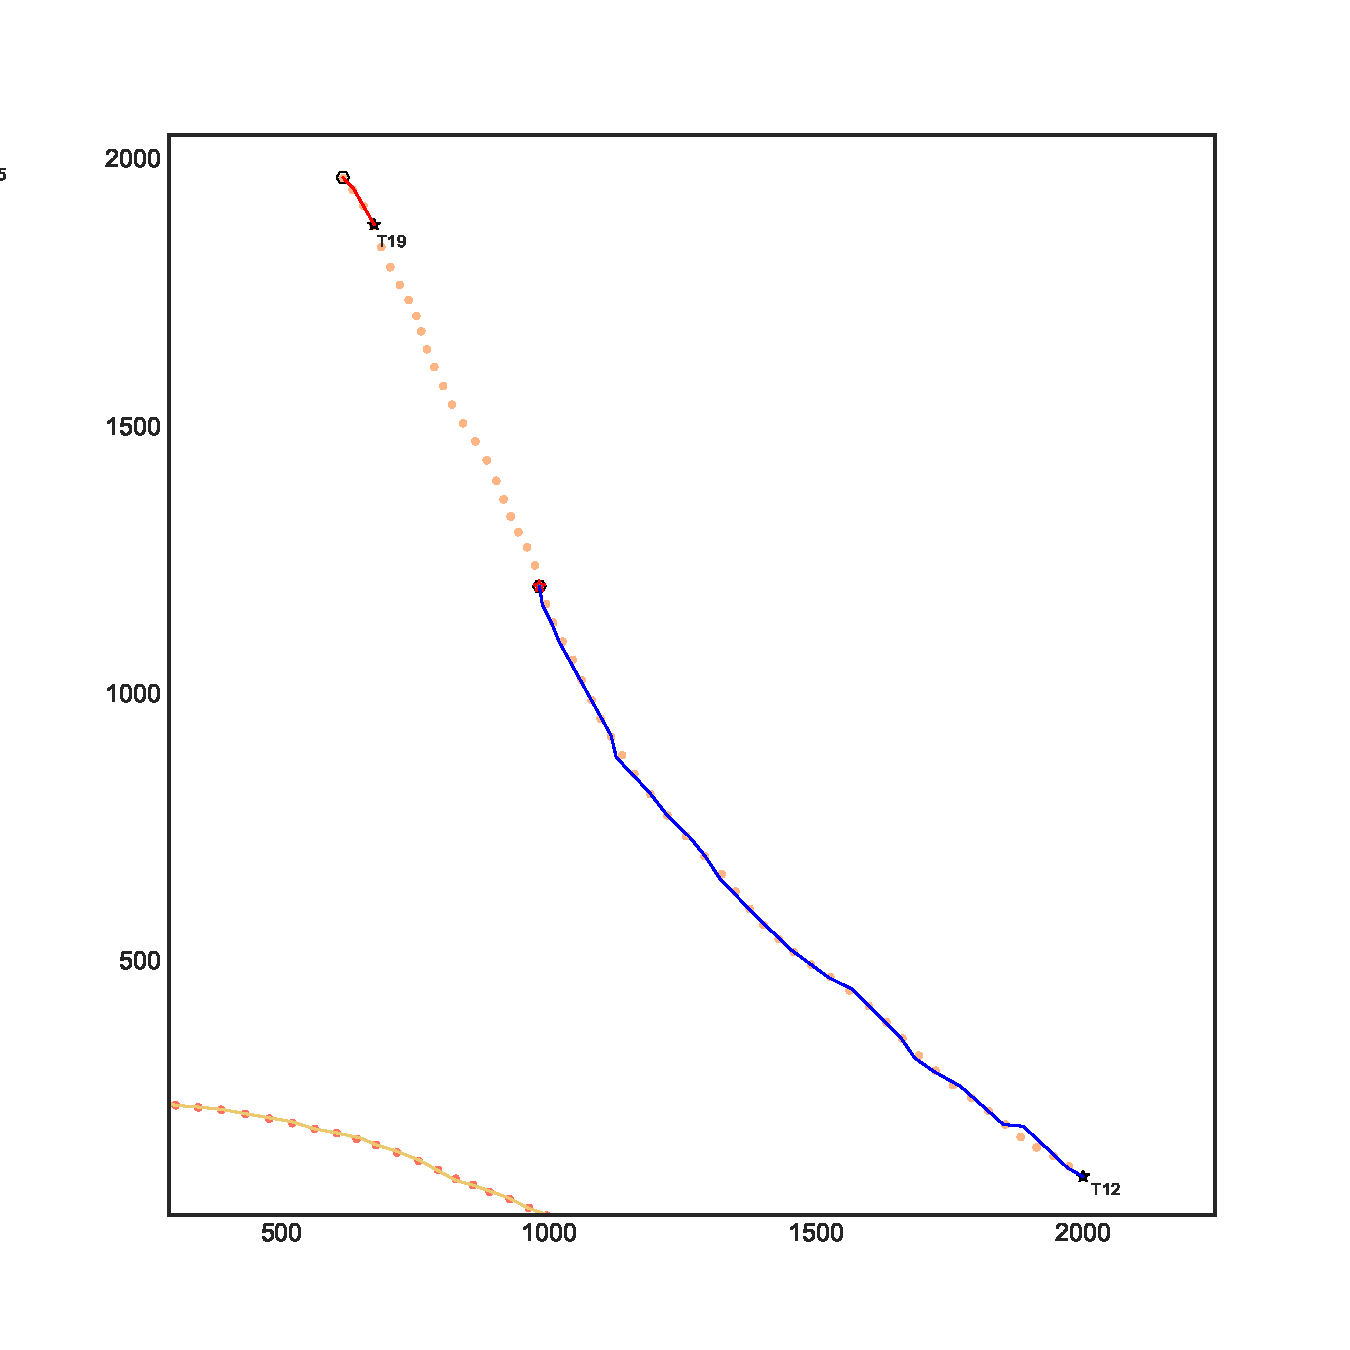
\includegraphics[width = .8\textwidth]{Figures/track_percentage_illustration.pdf}
\caption{Tracking percentage illustration}\label{fig:track_percentage}
\end{figure}

\section{Scenario}\label{sec:scenario}
All simulations in this work is based on a generated scenario, as shown in Figure~\ref{fig:test_scenario}, with black dots marking the initial time and position. The radar range is 5500 meter (~3 \glspl{nm_acr}), which gives an area of surveillance of approximately 95 square km. The scenario contains 16 targets, which all starts inside the observable area of the radar. The scenario contains a mixture of fast and slow moving vessels, some with sharp turns and some almost at stand still. Table~\ref{tab:init_states} shows the initial states of all targets, and the true path is generated once from these initial values.
\begin{figure}
\centering
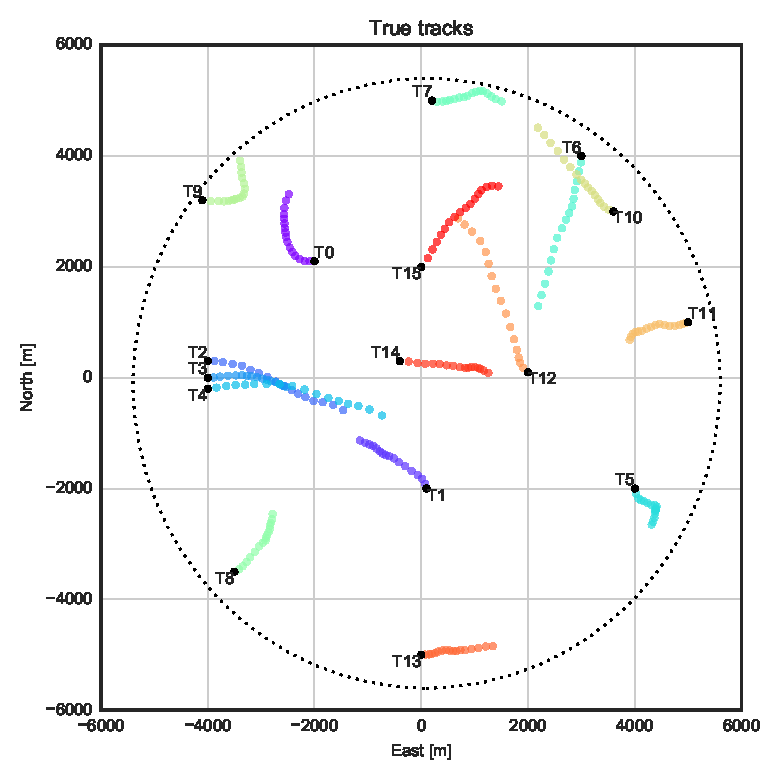
\includegraphics[width = .9\textwidth]{Figures/plots/ScenarioTruth.pdf}
\caption{True tracks}\label{fig:test_scenario}
\end{figure}
\begin{table}
\centering
\begin{tabular}{c c c c c}
\bfseries Target & \bfseries North & \bfseries East & \bfseries North speed & \bfseries East speed \\ 
\toprule
\csvreader[head to column names,respect percent=true]{{Figures/plots/Scenario_Initial_State.csv}}{}
{\T{} & \NP{} & \EP{} & \NS{} & \ES{} \\}
\end{tabular}
\caption{Initial states}\label{tab:init_states}
\end{table}

From this base scenario, five scenarios where generated with different AIS configuration on the vessels, see Table~\ref{tab:ais_scenarios}. The first scenario represent the baseline with only radar information available, whereas the rest have some level of AIS information. Scenario 1 adds three class B AIS transmitters, and is representing a situation where all the targets are smaller vessels with some voluntarily installed AIS transceivers. In scenario 3, all vessels have AIS class B installed. This scenario represents a best case situation regarding yacht and leisure vessels from an autonomous anti collision perspective and is only realistic if AIS class B where to be mandatory for these vessel classes. Scenario 2 is the same as scenario 1, with the difference that the vessels have class A transmitters in stead of class B. This gives them higher and smarter rate of transmission, which in theory should improve tracking under challenging conditions. This scenario can be viewed as a few commercial vessels travelling in between a large group of yachts. The last scenario, where all targets are equipped with class A transmitters is the ultimate situation for any fusion tracking system. This case would be realistic in a crowded professional working area, for instance harbours, fishing areas and off-shore installations.
\begin{table}
\centering
\csvautotabular{{Figures/plots/Scenario_AIS_State.csv}}
\caption{AIS scenario configuration}\label{tab:ais_scenarios}
\end{table}

\section{Simulation}
Both initialization- and tracking performance is averaged over a set of 50 Monte Carlo simulations with differently seeded clutter- and missed detections points. All simulations were done with a sampling interval at 2.5 seconds (24 \gls{rpm}), which is the most common rotation speed on a coastal maritime radar. Since early simulations showed that the variation between the different scenarios when analysing the initialization time and termination of false track were negligible. Based on this, only scenario 0 were used for initialization analysis to avoid excessive plot `duplicates'. Each of the 144 initialization variations and 240 track performance simulations where run 50 times with differently seeded clutter and misdetections on a dual Intel i7--6700 server running Linux Ubuntu with \gls{ssd} storage and 64 GB \gls{ram}.

\section{Initialization results}

%Figure: steady-state number of errounous tracks vs. clutter level x (m/n)



\section{Tracking results}

%Figure: track percentage of targets with AIS vs. without